\documentclass[portuguese]{textolivre}

% metadata
\journalname{Texto Livre}
\thevolume{18}
%\thenumber{1} % old template
\theyear{2025}
\receiveddate{\DTMdisplaydate{2024}{10}{18}{-1}}
\accepteddate{\DTMdisplaydate{2024}{11}{19}{-1}}
\publisheddate{\DTMdisplaydate{2025}{2}{23}{-1}}
\corrauthor{Jackson Wilke da Cruz Souza}
\articledoi{10.1590/1983-3652.2025.55346}
%\articleid{NNNN} % if the article ID is not the last 5 numbers of its DOI, provide it using \articleid{} commmand 
% list of available sesscions in the journal: articles, dossier, reports, essays, reviews, interviews, editorial
\articlesessionname{articles}
\runningauthor{Souza, Semcovici e Pardo}
%\editorname{Leonardo Araújo} % old template
\sectioneditorname{Daniervelin Pereira}
\layouteditorname{João Mesquita}

\title{Proposta de algoritmo de classificação automática de papéis semânticos em português no âmbito do modelo Abstract Meaning Representation}
\othertitle{Proposal of an algorithm for automatic classification of semantic roles in Portuguese within the Abstract Meaning Representation model}

\author[1]{Jackson Wilke da Cruz Souza~\orcid{0000-0003-1881-6780}\thanks{Email: \href{mailto:jackcruzsouza@gmail.com}{jackcruzsouza@gmail.com}}}
\author[2]{Pedro Semcovici~\orcid{0009-0008-8455-8509 }\thanks{Email: \href{mailto:pedrosemcovici@usp.br}{pedrosemcovici@usp.br}}}
\author[3]{Thiago Alexandre Salgueiro Pardo~\orcid{0000-0003-2111-1319 }\thanks{Email: \href{mailto:taspardo@icmc.usp.br}{taspardo@icmc.usp.br}}}
\affil[1]{Universidade Federal da Bahia,Instituto de Ciência, Tecnologia e Inovação, Camaçari, BA, Brasil.}
\affil[2]{Universidade de São Paulo, Escola de Artes, Ciências e Humanidades, São Paulo, SP, Brasil.}
\affil[3]{Universidade de São Paulo, Instituto de Ciências Matemáticas e de Computação, São Carlos, SP, Brasil.}

%\usepackage{calc,easyReview,enumitem,longtable,multirow,tabularx,ulem}
%\newcolumntype{Y}{>{\centering\arraybackslash\hsize=1\hsize}X}%Custom-made column type to ensure that the columns are of equal width and center-aligned
%\usepackage{enumitem,colortbl,multirow,longtable}
\usepackage{multirow}
\setlist[enumerate]{topsep=1ex, parsep=1ex}

\addbibresource{article.bib}

\begin{document}
\maketitle
\begin{polyabstract}
\begin{abstract}
  O nível semântico em Processamento de Linguagem Natural (PLN) apresenta desafios significativos devido à complexidade dos fenômenos, que são menos suscetíveis a descrições objetivas. Nem todas as abordagens linguísticas, como o modelo teórico de papéis semânticos proposto por \textcite{cançado2017}, são facilmente implementáveis em sistemas computacionais devido à sua variabilidade terminológica e metodológica. O modelo Abstract Meaning Representation (AMR) \cite{banarescu2013,weischedel2013} tem se destacado por oferecer uma representação clara da estrutura argumental, proporcionando explicabilidade tanto para humanos quanto para sistemas computacionais sobre como o sentido se organiza em sentenças de línguas naturais. Baseando-se no AMR, desenvolvemos um classificador automático de papéis semânticos. Utilizando técnicas de Aprendizado de Máquina, nosso classificador foi treinado e testado em um corpus multigênero em Português do Brasil. Realizamos dois experimentos: o primeiro comparando Argumentos 0 e 1, e o segundo comparando Argumentos de 0 a 4, obtendo melhores resultados no primeiro experimento. Os resultados ressaltam a importância da aplicação de modelos semânticos em PLN para o português e abrem possibilidades para novas iniciativas de pesquisas.

  
  

\keywords{Papéis semânticos \sep Abstract Meaning Representation \sep Processamento de Linguagem Natural}
\end{abstract}

\begin{english}
\begin{abstract}
  Semantic level in Natural Language Processing (NLP) presents significant challenges due to the phenomena’s complexity, which are less amenable to objective description. Not all linguistic approaches, such as the semantic role theory proposed by \textcite{cançado2017}, can be easily implemented in computational systems due to their terminological and methodological variability. The Abstract Meaning Representation (AMR) model \cite{banarescu2013,weischedel2013} has gained prominence for providing a clear representation of argument structure, offering explicability both for humans and computational systems on how meaning is organized in sentences of natural languages. Based on AMR, we developed an automatic semantic role classifier. Using Machine Learning techniques, our classifier was trained and tested on a multi-genre corpus in Brazilian Portuguese. We conducted two experiments: the first comparing Arguments 0 and 1, and the second comparing Arguments 0 to 4, achieving better results in the former. The results highlight the importance of applying semantic models in NLP for Portuguese and open possibilities for new research initiatives.
  
  
\keywords{Semantic roles \sep Abstract Meaning Representation \sep Natural Language Processing}  

\end{abstract}
\end{english}
\end{polyabstract}

\section{Introduction}\label{sec-intro}

Technology-assisted interpreting has experienced exponential growth in
recent years, reflected in the dizzying progress in the development of
information and communication technology (ICT) tools and resources
\cite{gutierrezArtacho2016,mezcua2019}. These innovative
technologies have greatly facilitated the interpretation and
comprehension of texts in different linguistic contexts \cite{olallaSoler2015}. In this sense, computer-assisted interpreting (CAI)
has become crucial in an increasingly globalised and connected society,
playing a pivotal role in breaking down language barriers and
facilitating effective communication in an environment characterised by
cultural and linguistic diversity \cite{mellinger2019,li2021}. In
response to the growing demand for instant online communication and the
need to overcome language limitations in a global environment, CAI has
established itself as an infallible tool for a wide range of
applications, from interpreting international business meetings to
translating multimedia content in real time \cite{fantinuoli2017a,alcaidemartinez2021}.

The integration of technology has revolutionised the way individuals
interact with language, opening new possibilities for increasing the
efficiency and accuracy of text interpretation, both in real time and
asynchronously \cite{gaber2023a,ramirezRodriguez2023}. The development
of ICT tools has led to improvements in natural language processing,
machine translation, speech recognition and other related technologies,
resulting in significant advances in text interpretation \cite{valeroGarces2024}. These tools have been particularly useful in overcoming language
barriers in multicultural environments, facilitating communication
between speakers of different languages and promoting intercultural
understanding \cite{perez2020}.

The use of CAI does, however, present certain difficulties. In the
phraseological domain, understanding idiomatic expressions remains a
significant challenge, as these linguistic constructions can be
particularly difficult to interpret accurately due to their cultural
embeddedness \cite{corpaspastorgaber2021,ramirezRodriguez2022}.
Cultural and contextual differences can lead to inaccurate or ambiguous
translations of these expressions, resulting in misunderstandings and
communication problems. In addition, CAI is often based on pre-defined
algorithms and databases, which can limit its ability to adapt to new
idioms and emerging expressions \cite{ortigoza2024}. This problem
identified in the interpretation of idiomatic expressions by CAI adds to
the previously mentioned challenges in technology-assisted phraseology,
where accuracy and fluency in the interpretation of texts in different
linguistic contexts are key to effective communication. The complexity
of idiomatic expressions, such as idioms, and their culturally
contextual nature require new approaches and specialised tools to
improve the interpretation of such expressions, which represents a
relevant area of research in the development of technology-assisted
phraseology.
\section{Revisão da literatura}\label{sec-revisão}

Nesta seção, serão apresentados trabalhos recuperados da literatura que
dialogam direta ou indiretamente com a temática desenvolvida nesta
pesquisa, sobretudo relacionados aos papéis semânticos em PLN e à
aplicação de SRL.

\subsection{Papéis semânticos nos estudos de PLN}\label{sub-sec-papeissemanticos}

Segundo \textcite{banarescu2013}, o modelo AMR objetiva capturar e
representar explicitamente aspectos do significado de uma sentença. Esse
modelo teórico propõe a enumeração de argumentos na tentativa de
simplificar a proposta de papéis semânticos. \textcite{weischedel2013} apontam que na AMR, tradicionalmente, segue-se a seguinte
proposta:

\begin{itemize}
\item[Arg0]\label{arg0}: refere-se ao argumento da ação que desempenha o papel de agente;
\item[Arg1]\label{arg1}: refere-se ao argumento principal que é afetado pela ação
  expressa pelo verbo, correspondendo, em geral, ao objeto direto;
\item[Arg2]\label{arg2}: refere-se a um argumento secundário ou ao objeto indireto em
  construções que apresentam verbos;
\item[Arg3, Arg4 e Arg5]\label{arg345}: são termos menos frequentes nas construções
  linguísticas, ocorrendo em construções verbais mais complexas, como
  para o verbo ``dar'' ou ``entregar''.
\end{itemize}

A partir dessas definições, é importante ressaltar que a proposta do
modelo AMR pode ou não levar em conta aspectos morfossintáticos e/ou a
ordem em que os itens lexicais ocorrem nas sentenças. O Arg0, por
exemplo, é definido apenas a partir de aspectos semânticos; todos os
outros argumentos levam em conta, em alguma medida, informações
gramaticais que consideram a ordem e/ou a classificação morfossintática.
Outro ponto importante desse modelo é que itens lexicais/\emph{tokens}
que não contribuem fortemente para a construção dos sentidos em
determinadas sentenças (como determinantes/artigos) não são considerados
na análise, dando-se ênfase na estrutura argumental.

A título de exemplificação, tem-se a sentença apresentada em \ref{itm3}, que
foi extraída do \emph{corpus} AMR-PT \cite{inacio2023}, que
contempla sentenças extraídas da obra ``O pequeno príncipe'', dentre
outros gêneros textuais, atualmente.

\begin{enumerate}[start=3,label={(\arabic{enumi})}]
    \item\label{itm3} Meu desenho não representava um chapéu.
\end{enumerate}

De acordo com a proposta AMR, na sentença exemplificada em \ref{itm3}, tem-se
dois argumentos: ``desenho'' é o argumento principal em relação ao verbo
``representar'' e, por isso, recebe a classificação de Arg1; e
``chapéu'', que desempenha o papel de ``objeto'', recebe a classificação
Arg2. Os itens lexicais ``meu'' e ``não'' indicam, respectivamente, a
relação de posse e a polaridade negativa da sentença. Tais relações
também são consideradas e representadas no modelo AMR. Por fim, o item
``um'' não faz parte da estrutura argumental pois não exerce modificação
significativa sobre ``chapéu'', ainda que desempenhe função de
indeterminação sobre ele.

Além disso, o modelo propõe possibilidades de representação do
conhecimento semântico, aspecto extremamente importante para
implementação computacional. Uma dessas representações é a
\emph{estrutura de grafos}, em que os nós representam eventos e
entidades mencionados na sentença; já as arestas representam as relações
entre os nós. A \Cref{fig-01} representa a estrutura argumental do exemplo em \ref{itm3}.

\begin{figure}[h]
  \centering    
  \begin{minipage}{.75\textwidth}
  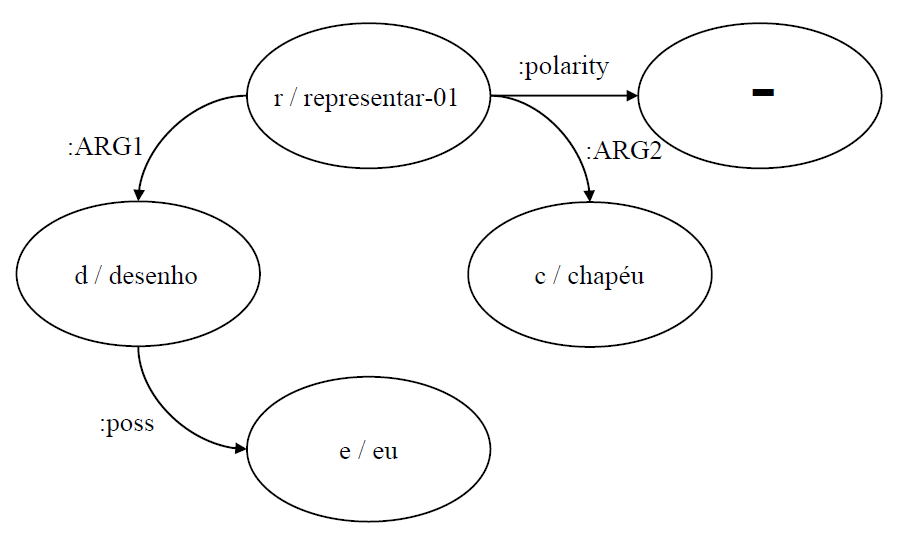
\includegraphics[width=\textwidth]{figure01.png}
  \caption{Exemplo de grafo AMR.}
  \label{fig-01}
  \source{Adaptado de \textcite{anchiêta2022}.}
  \end{minipage}
\end{figure}

Outra possibilidade de representação é por meio de \emph{notação lógica}
(\Cref{fig-02}), em que, a partir da identificação léxica do predicado,
apontam-se os tipos de argumentos, seus respectivos itens lexicais e a
relação semântica estabelecida entre eles. Por fim, na \emph{notação
Penman} (\Cref{fig-03}), feita em formato textual, há delimitação de
instâncias, que são os itens lexicais que funcionam como argumentos e/ou
predicados nas sentenças, a estrutura argumental entre as instâncias e
as relações que podem estabelecer entre si. Cabe destacar que as três
figuras equivalem à mesma representação semântica, sendo que a \Cref{fig-01},
por seu apelo gráfico, pode ser melhor interpretável por humanos, ao
passo que as Figuras 2 e 3 permitem implementações computacionais por
serem notações lógicas.

\begin{figure}[h]
\begin{minipage}{.45\textwidth}
  \centering
  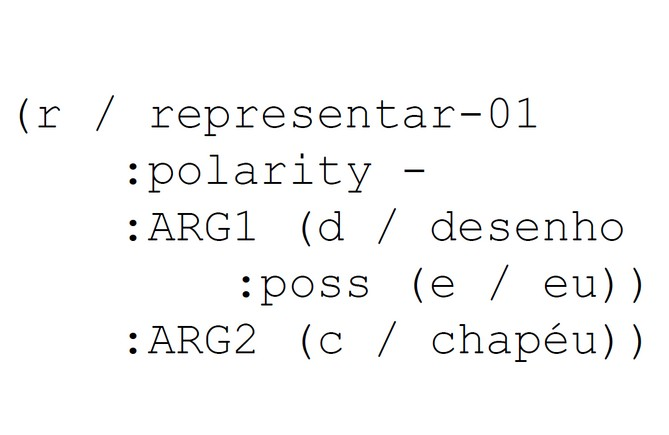
\includegraphics[width=\textwidth]{figure02.jpg}
  \caption{Exemplo de notação lógica no modelo AMR.}
  \label{fig-02}
  \source{Elaborado pelos autores.}
\end{minipage}%
\hfill
\begin{minipage}{.45\textwidth}
  \centering
 
\includegraphics[width=\textwidth]{figure03.jpg}
  \caption{Exemplo de notação Penman no modelo AMR.}
  \label{fig-03}
  \source{Elaborado pelos autores.}
\end{minipage}
\end{figure}

Outro aspecto importante na proposta do modelo é a classificação dos
conceitos. De acordo com \textcite{anchiêta2022}, os conceitos AMR podem
ser classificados em \emph{concretos} (palavras em suas formas
lexicalizadas, como ``mulher'' e ``homem''), \emph{framesets} do
\emph{Proposition Bank} -- PropBank\footnote{PropBank pode ser definido
  como um recurso de sentenças anotadas com funções semânticas
  \cite{jurafsky2023}. Por conta da dificuldade de se obter um
  conjunto ``universal'' de papéis semânticos, como demonstrados nesta
  seção, nos PropBanks convencionou-se que as relações semânticas são
  numeradas (ao invés do uso de seus nomes), que é justamente a
  filosofia adotada pela AMR.} -- \cite{palmer2005} ou
\emph{abstratos} (que não correspondem a nenhuma unidade lexical das sentenças, como ``\%'' e ``endereço de e-mail'', por exemplo).

\subsection{Trabalhos relacionados à SRL}\label{sub-sec-trabalhos}

De acordo com \textcite{hartmann2017}, SRL é uma tarefa em PLN
que detecta eventos descritos em sentenças e os participantes desses
eventos. Os eventos ocorrem nas sentenças sob formas morfológicas de
verbos, nomes, adjetivos e advérbios; porém, a classe que mais é
explorada na literatura é a dos verbos, pois expressam eventos, além de
ser impossível construir orações completas com ausência de verbos. As
demais classes de palavras não expressam eventos da mesma forma que os
verbos, nem em proporção.

Ainda segundo \textcite{hartmann2017}, os métodos empregados na
anotação automática de papéis semânticos são, na maioria, com base em
AM. Nesse contexto, é necessário que haja \emph{corpora} linguísticos
anotados para que os algoritmos de AM possam ser treinados e avaliados
quanto ao desempenho da tarefa a que eles foram submetidos. A literatura
aponta alguns \emph{corpora} disponíveis com anotação AMR, importantes
para as tarefas de SRL, a saber: \textcite{xue2014} para o inglês;
\textcite{vanderwende2015} com uma abordagem multilíngue para
Francês, Alemão, Espanhol e Japonês; \textcite{damonte2019} %\alert{Damonte e Cohen (2018)} 
para as línguas italiana, espanhola, alemã e chinesa; \textcite{migueles2018} especificamente para o espanhol; e \textcite{anchiêta2018} e
\textcite{inacio2023}, para o PB. Destaca-se que há também
recursos com papéis semânticos desvinculados da estruturação completa
proposta pela AMR, como é o caso do PropBank do inglês, citado
anteriormente, e o PropBank.Br \cite{duran2012} e o recente PBP
(\emph{Porttinari-base Propbank}) para o português \cite{freitas2024}.

Em especial, o \emph{corpus} para o PB é composto por sentenças anotadas
com o modelo AMR para diferentes gêneros textuais. A primeira versão do
\emph{corpus} apresentava sentenças extraídas do romance ``O pequeno
príncipe'', tido como \emph{corpus} ``\emph{little prince}''. Em sua
segunda versão, o escopo de domínio foi ampliado para notícias extraídas
do jornal Folha de S. Paulo \cite{duran2012}, tido como o
\emph{corpus} ``\emph{news}''. Em sua versão mais recente\footnote{Disponível
  em: \href{https://github.com/nilc-nlp/AMR-BP}{GitHub -
  nilc-nlp/AMR-BP}. Acesso em: 20 jul.2024.}, o AMR-PB apresenta textos
opinativos, tido como \emph{corpus} ``\emph{opisums}'', e científicos,
tido como \emph{corpus} ``\emph{sci}''. Ademais, todos os \emph{corpora}
apresentam sentenças anotadas, identificando os papéis semânticos
seguindo a metodologia do PropBank.Br \cite{duran2012}.

Com relação ao PropBank.Br, \textcite{duran2012} destacam que o
\emph{corpus} é um repositório de proposições, alinhando-se ao que
\textcite{fillmore1968} apresenta sobre a estrutura base de uma frase, a saber:
um conjunto de relações entre substantivos e verbos, sem modificadores
de tempo, negação, aspecto e modo. Segundo as autoras, os verbos recebem
um código que indica seu sentido com relação ao \emph{frame} em que a
sentença está associada; já os argumentos são anotados com rótulos de
função numerados (de Arg0 a Arg5) e os modificadores são anotados com
rótulos de função ArgMs (Modificadores de argumento).

Vale a pena ressaltar que os \emph{corpora} delimitados aqui seguem as
diretrizes da literatura quanto ao PLN. Os conjuntos de dados
linguísticos acompanham os apontamentos de \textcite{gildea2002}, já
que representam semanticamente os papéis temáticos distanciando-se de
detalhamentos analíticos, ao passo que se aproximam da objetividade e
simplificação de rótulos para garantir melhor desempenho no processo de
classificação automática.

Partindo de \emph{corpora} anotados, é possível aplicar diferentes
técnicas de AM. O trabalho de \textcite{hartmann2015} realizou a análise
automática de papéis semânticos utilizando AM nos \emph{subcorpora news}
e \emph{opisums}. Aplicando diferentes abordagens (utilizando ou não
árvores sintáticas treinadas), os autores obtiveram Medida-F de 87,8\%
para o \emph{corpus news}, e 94,5\% para o \emph{corpus opisums}.

Hartmann, \textcite{duran2012} realizaram a avaliação de dois sistemas
de SRL para textos jornalísticos. O sistema desenvolvido por \textcite{fonseca2013} teve o propósito de anotar automaticamente os papéis
semânticos para o PB, sem lançar mão de ferramentas de PLN externas ao
sistema desenvolvido; os resultados dessa avaliação indicam uma Medida-F
de 68\%. Já o sistema de \textcite{alva-manchego2012} empregou a abordagem
supervisionada de AM e obteve Medida-F de 79,6\%. Destaca-se que ambos
os trabalhos foram baseados no \emph{corpus} PropBank.Br.

\textcite{ilmy2021} realizaram a análise de frases em indonésio
utilizando a AMR com abordagem de aprendizado de máquina. Inspirado no
trabalho de \textcite{zhang2019}, o sistema desenvolvido por \textcite{ilmy2021} compreende três etapas: (i) previsão de pares de palavras, (ii)
previsão de rótulos e (iii) construção de grafos. Em (i), utiliza-se um
componente de análise de dependência para obter as conexões entre
palavras. Em (ii), emprega-se um algoritmo de aprendizado supervisionado
para prever os rótulos entre as conexões. Em (iii), a partir dos rótulos
previstos, é criado o grafo da sentença em AMR. Avaliado com uma base de
dados de frases simples coletadas de artigos e notícias, o modelo
atingiu uma pontuação SMATCH\footnote{SMATCH é uma métrica que tem como
  objetivo avaliar estruturas semânticas em ocorrências linguísticas
  \cite{cai2013}.} de 0,820.

\section{Metodologia}\label{sec-metodologia}

Não foi necessária uma análise ética prévia por parte dos conselhos de
projetos adequados para a investigação, uma vez que os participantes não
foram identificados. Por não haver conflito de interesses, a Texto Livre
não terá quaisquer consequências, inclusive assistência integral e
eventual, ressarcimento de qualquer dano resultante a qualquer dos
participantes da pesquisa, conforme a Resolução nº 510, de 7 de abril de
2016, do Conselho Nacional de Saúde do Brasil.

A metodologia é a explicação minuciosa, detalhada, rigorosa e exata de
toda a ação desenvolvida no método de trabalho da pesquisa \cite{lakatos2003}. A pesquisa é um estudo de caso, que teve o aluno como
objeto de estudo. \textcite[p. 32]{yin2005} argumenta que o estudo de caso visa a \enquote{conhecer em profundidade o como e o porquê de uma determinada
	situação que se supõe ser única em muitos aspectos, procurando descobrir
	o que há nela de mais essencial e característico}. O estudo de caso é
caracterizado pelo estudo profundo e exaustivo de um ou poucos objetos,
de maneira a permitir o seu conhecimento amplo e detalhado. O caso
experimental caracteriza-se por determinar um objeto de estudo,
selecionar as variáveis que seriam capazes de influenciá-lo, definir as
formas de controle e de observação dos efeitos que a variável produz no
objeto \cite{gil2002}. A coleta dos dados foi realizada em uma escola
secundária do sul de Moçambique. Fizeram parte da amostra 50 alunos do
ensino secundário, selecionados de forma aleatória, dos quais 25
participaram do estudo das PO e aplicação do Q3DM. Os restantes 25
estiveram envolvidos no estudo das SCs e aplicação do GeoGebra. Em ambos
os estudos, todos os alunos experimentaram as aplicações (Q3DM ou
GeoGebra). A pesquisa apresenta um estudo de caso interpretativo, o qual
desenvolve categorias conceituais indutivamente para examinar os
pressupostos iniciais, as intenções e significados das ações e
expressões dos alunos \cite{amado2017}. A compreensão interpretativa é
sustentada a partir do relato pormenorizado da interação dos sujeitos em
seu meio natural \cite{coulon1995}. A visão interpretativa descreveu as
ações dos alunos em ambiente de sala de aula e os significados das ações
no processo de toda a pesquisa \cite{coutinho2011}.

Foi possível, pois, observar e interpretar tudo o que ocorreu, tornando
viável a análise das relações causa-efeito. Foi possível , também,
qualificar as ações dos alunos em todo o processo de aprendizagem, por
meio das interpretações dos significados de seus comportamentos durante
a mediação da aula e as respostas do questionário de satisfação. Além
disso, os dados foram coletados por meio das técnicas de observação do
participante, com tomada de notas e de registro fotográfico, assim como
dos instrumentos de coleta de dados aplicados, como os questionários de
satisfação.

\subsection{Realização das aulas}\label{sub-sec-Realização das aulas}

As aulas consistiram na apresentação de dois temas, PO e SCs, de forma
separada. Para os alunos da 9ª classe, o tema de pesquisa foi PO, e foi
utilizado o Q3DM. A professora primeiramente apresentou o tema,
explicando o que eram POs, dizendo que eram figuras geométricas sobre um
plano que poderiam ser comparadas à sombra do mesmo objeto no horário em
que o sol estaria no ponto mais alto no dia. Depois, demonstrou as
vistas ortogonais do sólido. (Ver \Cref{fig-03}).

\begin{figure}[htpb]
\centering
\begin{minipage}{.5\textwidth}

\includegraphics[width=\textwidth]{figures/figure03.jpg}
\caption{Vistas ortogonais e ortográficas: vista frontal; vista superior; e vista lateral esquerda.}
\label{fig-03}
\source{\url{http://turmag1215vialonga.blogspot.com/2014/10/projecoes-ortogonais.html}.}
\end{minipage}
\end{figure}

Posteriormente a professora apresentou a aplicabilidade das POs, dizendo
que eram destinadas à planificação de vários objetos. Com o auxílio das
simulações computacionais, construiu os sólidos geométricos e demonstrou
suas vistas ortogonais, apresentando os procedimentos para a manipulação
do Q3DM. (Ver \Cref{fig-04})

\begin{figure}[htpb]
\centering
\begin{minipage}{.5\textwidth}
\includegraphics[width=\textwidth]{figures/figure04.jpg}
\caption{Manipulação no Q3DM.}
\label{fig-04}
\source{Elaboração própria.}	
\end{minipage}
\end{figure}


A manipulação no Q3DM é feita por meio de cubos chamados Qubes, que
facilitam a criação e a montagem de objetos em três dimensões,
utilizando elementos digitais que podem ser inseridos, removidos,
deslocados, ampliados, inclinados, moldados geometricamente, girados e
coloridos.

Para os alunos da 12ª classe, o tema de pesquisa foi SCs e foi utilizado
o GeoGebra. A professora iniciou com a apresentação do tema SCs de
cilindro, explicando que a seção cilíndrica é uma figura resultante de
um plano secante no cilindro. A professora acrescentou que existem duas
situações distintas: quando o plano secante é paralelo ao eixo central
do cilindro; e quando o plano secante não é paralelo ao eixo central do
cilindro (ver as figuras \Cref{fig-05} e \Cref{fig-06}).

\begin{figure}[htpb]
\centering
\begin{minipage}{.25\textwidth}
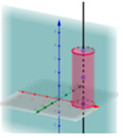
\includegraphics[width=\textwidth]{figures/figure05.jpg}
\caption{Secção paralela ao eixo central do cilindro.}
\label{fig-05}
\source{Elaboração própria.}
\end{minipage}
\end{figure}

\begin{figure}[htpb]
\centering
\begin{minipage}{.5\textwidth}
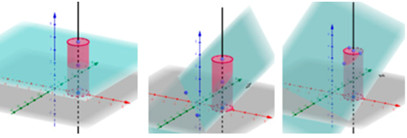
\includegraphics[width=\textwidth]{figures/figure06.jpg}
\caption{Secção não paralela ao eixo central do cilindro.}
\label{fig-06}
\source{Elaboração própria.}
\end{minipage}
\end{figure}

A professora, primeiramente, apresentou os diferentes posicionamentos
dos planos em relação ao eixo central do cilindro. Em seguida, com o
auxílio da tecnologia, apresentou à turma o software de geometria
dinâmica GeoGebra, indicando as funcionalidades de suas ferramentas e
como construir do ponto até o plano secante, com a ajuda dos
procedimentos para a sua manipulação no GeoGebra. Os alunos simularam as
SCs com o plano de nível; eles apresentaram-se atentos e motivados em
aprender a resolver o exercício no GeoGebra, particularmente para os
rapazes, os quais procuravam descobrir como construir diferentes sólidos
geométricos e como simular as VOs (vistas ortogonais).

\subsection{Realização do questionário}\label{sub-sec-Realização do questionário}

O questionário de satisfação aplicado teve como objetivo compreender se
o Q3DM e o GeoGebra facilitaram a aprendizagem das POs e SCs, e se o
\textit{smartphone} foi fácil de manipular. Ambos os questionários foram
preenchidos em 10 minutos. As questões visavam a coletar, nos dois
estudos, várias opiniões, incluindo: (1) se os aplicativos tecnológicos
facilitaram as representações 3D; (2) qual é a opinião deles sobre os
benefícios de usar os aplicativos ou se seria melhor resolver de forma
tradicional; (3) se os aplicativos são fáceis e intuitivos de usar; (4)
quais foram os aspectos positivos e negativos da aula; e, (5) como eles
classificariam a aprendizagem com o auxílio dos aplicativos.

\section{Resultados e discussão}\label{sec-resultados}

Como dito anteriormente, foram feitos dois experimentos de classificação
de papéis semânticos. O primeiro envolve uma classificação binária (Arg0
e Arg1); já o segundo aborda uma classificação multiclasse com cinco
rótulos (Arg0, Arg1, Arg2, Arg3 e Arg4). Na \Cref{tab-03}, apresentamos os
resultados obtidos, considerando as medidas P, R, MF e A.

\begin{table}[htbp]
  \centering 
  \begin{threeparttable}
  \caption{Resultados para os dois experimentos de classificação.}
  \label{tab-03}
  \begin{tabular}{*{9}{l}}
  \toprule
  \multirow{2}{*}{CLASSES} & \multicolumn{8}{c}{EXPERIMENTOS} \\
    & \multicolumn{4}{c}{1º experimento (Arg0 e Arg1)} & \multicolumn{4}{c}{2º experimento (Arg0 a Arg4)} \\
    & P & R & MF & A & P & R & MF & A \\
  Arg0 & 0,83 & 0,82 & 0,82 & 0,85 & 0,82 & 0,79 & 0,81 & 0,76 \\
  Arg1 & 0,88 & 0,89 & 0,88 & 0,85 & 0,77 & 0,84 & 0,80 & 0,76 \\
  Arg2 &  -   &   -  &   -  &  -   & 0,40 & 0,32 & 0,36 & 0,76 \\
  Arg3 &  -   &   -  &   -  &  -   & 0,33 & 0,14 & 0,20 & 0,76 \\
  Arg4 &  -   &   -  &   -  &  -   & 1,00 & 0,20 & 0,33 & 0,76 \\
  \bottomrule
  \end{tabular}
  \source{Elaborado pelos autores.}
  \end{threeparttable}
\end{table}

Para o primeiro experimento, os resultados mostram um desempenho
equilibrado entre as duas classes. As métricas P, R e MF para Arg0 são,
respectivamente, 83\%, 82\% e 82\%, enquanto para Arg1 são 88\%, 89\% e
88\%. Esses resultados indicam um classificador bem balanceado,
sugerindo que o modelo consegue distinguir bem entre essas duas classes.

Por haver um aumento de classes, já era esperado um desbalanceamento na
performance do modelo entre as diferentes classes, no segundo
experimento. Para as classes Arg0 e Arg1, os resultados são semelhantes
aos do primeiro experimento, com MF de 81\% e 80\%, respectivamente. No
entanto, para as outras classes (Arg2, Arg3 e Arg4), as métricas são
significativamente mais baixas.

Para a classe Arg2, as medidas P, R e MF são 40\%, 32\% e 36\%,
respectivamente. A classe Arg4 apresenta uma precisão perfeita (100\%),
mas uma revocação extremamente baixa (20\%), resultando em uma MF de
apenas 33\%. A classe Arg3 também apresenta baixos valores em todas as
métricas, com precisão, revocação e medida F de 33\%, 14\% e 20\%,
respectivamente.

A acurácia de 76\% no segundo experimento sugere que o modelo tem uma
alta taxa de acertos nas classes majoritárias (Arg0 e Arg1), mas tem
dificuldade para classificar corretamente as classes minoritárias (Arg2,
Arg3 e Arg4), o que é evidenciado pelo baixo desempenho nestas classes.
Esse desbalanceamento indica que o modelo pode tender a classificar mais
exemplos nas classes majoritárias, possivelmente devido a um número
insuficiente de exemplos das classes minoritárias durante o treinamento.

Esse resultado pode ser justificado não apenas do ponto de vista
computacional, perpassado pelo desbalanceamento das classes, mas também
de uma perspectiva linguística. No primeiro experimento, consideraram-se
papéis de argumentos mais prototípicos e mais claramente associados a
posições sintáticas estabelecidas como sujeito e objeto, sendo mais
fáceis de se classificar. Já no segundo, observa-se uma diversidade
semântica e estrutural, sendo argumentos menos prototípicos, ocasionando
equívocos de classificação de predicados e adjuntos como argumentos.
Nesse caso, parece pertinente pontuar que é quase impossível desassociar
a estrutura argumental da sintaxe, cabendo mais discussões sobre essa
correlação em estudos posteriores.

Na língua geral, os papéis Arg0, Arg1 e Arg2 (como exemplificado em \ref{itm5a}, \ref{itm5b} e \ref{itm5c}, respectivamente) são mais profícuos, e os falantes constroem
rotineiramente sentenças que cumprem essas estruturas argumentais. Já as
construções que apresentam Arg3 e Arg4 (como exemplificado em \ref{itm5d} e \ref{itm5e},
respectivamente) seguem a proporção inversa. Destaca-se que os exemplos
demonstrados em \ref{itm5} foram extraídos do \emph{corpus little prince}, já
anotado com o modelo AMR, tendo a indicação do argumento correspondente
em foco.


\begin{enumerate}[start=5,label={(\arabic{enumi})}]
  \item\label{itm5}
    \begin{enumerate}[label=(\arabic{enumi}.\alph*)]
      \item\label{itm5a} {[}Ela{]}\textbf{\textsubscript{Arg0}} me perfumava.
      \item\label{itm5b} Perdoa-me {[}(eu){]}\textbf{\textsubscript{Arg1}}.
      \item\label{itm5c} Mas era tão {[}comovente!{ ]}\textbf{\textsubscript{Arg2}}
      \item\label{itm5d} {[}Perfura-o{]}\textbf{\textsubscript{Arg3}} com suas raízes.
      \item\label{itm5e} Vou passear até a {[}vinha.{]}\textbf{\textsubscript{Arg4}}
    \end{enumerate}
\end{enumerate}

É importante ressaltar que os predicados no modelo AMR equivalem à
descrição de uma ação, evento, estado ou relação e, por isso, são
frequentemente associados aos verbos, ainda que seja possível
associá-los a adjetivos e/ou substantivos. Além disso, frequentemente os
predicados correspondem a \emph{frames} semânticos, construindo cenas e
relações que exigem certos complementos. Já os argumentos são partícipes
ou entidades que se relacionam aos predicados, respondendo a perguntas
como ``quem'', ``o que?'' e ``para quem?'', por exemplo, sendo
enumerados em função da posição nos \emph{frames} em que são evocados.

Partindo desse princípio, os exemplos \ref{itm5a}, \ref{itm5b} e \ref{itm5e} cobrem essa
concepção; ainda que o quinto exemplo seja, na teoria linguística, um
argumento da preposição, na perspectiva da AMR ele é um argumento do
\emph{frame} ``passear''. Ao analisar os exemplos presentes em \ref{itm5c} e
\ref{itm5d}, evoca-se a necessidade de realizar revisões da anotação realizada.
Em \ref{itm5c}, ``comovente'' deveria ser considerado como predicado, mas
recebeu a anotação de argumento, pois completa o sentido de estado
(``ser comovente'', no caso). Já em \ref{itm5d}, o argumento deveria ser apenas
o objeto direto (no caso, ``o'') e não o verbo ``perfurar''. Esta última
colocação é justificada por uma questão de tokenização do \emph{corpus}
e do modelo de segmentação morfossintática utilizado, aglutinando o
``o'' a ``perfura''.

Ainda, em seus estudos, \textcite{cançado2009} encontrou predicados com no
máximo cinco lugares, como o verbo \emph{transportar} em ``João
transportou os livros no carro de São Paulo para a Bahia''. Nesse caso,
a autora admite que o complemento locativo ``no carro'' não é parte
obrigatória da estrutura argumental.

Nesse sentido, parece pertinente observar não apenas o quanto os
classificadores propostos acertam, mas também como se distribui o
equívoco de classificação no conjunto de dados. Por conta disso, foi
feita uma análise sobre a matriz de confusão dos modelos criados, em que
é possível avaliar a performance dos modelos em função de verdadeiros e
falsos positivos e negativos. Apresentamos as matrizes de confusão para
os dois experimentos nas \Cref{fig-04,fig-05}.


\begin{figure}[htpb]
\begin{minipage}{.45\textwidth}
  \centering
  \includegraphics[width=\textwidth]{figure04.jpg}
  \caption{Matriz de confusão do primeiro experimento}
  \label{fig-04}
  \source{Elaborado pelos autores.}
\end{minipage}%
\hfill
\begin{minipage}{.45\textwidth}
  \centering
  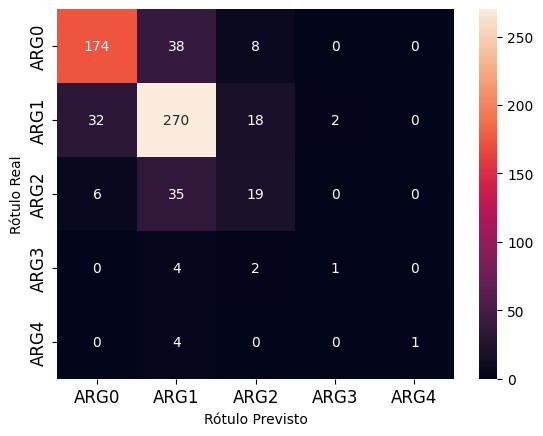
\includegraphics[width=\textwidth]{figure05.jpg}
  \caption{Matriz de confusão do segundo experimento}
  \label{fig-05}
  \source{Elaborado pelos autores.}
\end{minipage}
\end{figure}

As matrizes de confusão para os dois experimentos complementam as
métricas de avaliação apresentadas. No primeiro experimento, o modelo
mostra um bom equilíbrio entre P e R, com 179 (de 219) exemplos de Arg0
e 286 (de 323) exemplos de Arg1 corretamente classificados.

No segundo experimento, o modelo apresentou desequilíbrio em seu
desempenho. As classes Arg0 e Arg1 mantêm uma alta taxa de acerto, ao
passo que Arg2, Arg3 e Arg4 sofrem de baixa precisão e alta taxa de
erros. Essa confusão se deve ao fato de haver um desbalanceamento entre
os tipos de argumentos, conduzindo à classificação conforme a classe
majoritária, a saber, Arg1, conforme já discutido anteriormente.

Ainda, foi feita uma análise sobre o desempenho do modelo considerando
as classes e os \emph{corpora} utilizados nos dois experimentos.

\begin{table}[htpb]
  \centering
  \begin{threeparttable}
    \caption{Resultados do Experimento 1 em função dos \emph{corpora} utilizados.}
    \label{tab-04}
    \begin{tabular}{*{6}{l}}
      \toprule
      Corpora & Classe & P & R & MF & \multicolumn{1}{>{\raggedright\arraybackslash}p{2cm}}{Qnt. de instâncias} \\
      \midrule
      \arrayrulecolor[gray]{.7}
      \multirow{2}{*}{\emph{little prince}} 
        & Arg0 & 0,89 & 0,87 & 0,88 & 119 \\
        & Arg1 & 0,90 & 0,91 & \textbf{0,91} & 151 \\
      \midrule
      \multirow{2}{*}{\emph{news}} 
        & Arg0 & 0,74 & 0,75 & 0,74 & 60 \\
        & Arg1 & 0,87 & 0,86 & \textbf{0,87} & 116 \\
      \midrule
      \multirow{2}{*}{\emph{opisums}} 
        & Arg0 & 0,77 & 0,71 & 0,74 & 34 \\
        & Arg1 & 0,78 & 0,84 & \textbf{0,81} & 43 \\
      \midrule
      \multirow{2}{*}{\emph{sci}} 
        & Arg0 & 0,86 & 1,00 & 0,92 & 6 \\
        & Arg1 & 1,00 & 0,92 & \textbf{0,96} & 13 \\
      \arrayrulecolor{black}
      \bottomrule
    \end{tabular}
    \source{Elaborado pelos autores.}
  \end{threeparttable}
\end{table}

Na \Cref{tab-04}, relativa ao Experimento 1, observa-se que, considerando a
medida de avaliação MF, o modelo apresenta um melhor desempenho para
classificar Arg1 do que Arg0 para todos os \emph{corpora} utilizados.
Tal resultado pode ser explicado pela quantidade de instâncias
analisadas em Arg1 ser maior que Arg0. Ainda sobre a distribuição das
instâncias entre os \emph{corpora}, destaca-se que, apesar do
\emph{corpus sci} apresentar menos instâncias (no total, 19), o
\emph{corpus opisums} apresentou o menor desempenho com relação a MF, a
despeito da quantidade de instâncias (no total, 77). No entanto, é
possível notar que há um bom equilíbrio entre P e R para todos os
\emph{corpora}, indicando resultados consistentes para a classificação
do modelo.

\begin{table}[htpb]
  \centering
  \begin{threeparttable}
    \caption{Resultados do Experimento 2 em função dos \emph{corpora} utilizados.}
    \label{tab-05}
    \begin{tabular}{*{6}{l}}
      \toprule
      Corpora & Classe & P & R & MF & \multicolumn{1}{>{\raggedright\arraybackslash}p{2cm}}{Qnt. de instâncias} \\
      \midrule
      \arrayrulecolor[gray]{.7}
      \multirow{5}{*}{\emph{little prince}} 
        & Arg0 & 0,85 & 0,89 & \textbf{0,87} & 120 \\
        & Arg1 & 0,81 & 0,82 & 0,81 & 151 \\
        & Arg2 & 0,22 & 0,19 & 0,21 & 21 \\
        & Arg3 & 0,50 & 0,20 & 0,29 & 5 \\
        & Arg4 & 1,00 & 0,25 & 0,40 & 4 \\
      \midrule
      \multirow{5}{*}{\emph{news}} 
        & Arg0 & 0,77 & 0,68 & 0,73 & 60 \\
        & Arg1 & 0,74 & 0,86 & \textbf{0,80} & 115 \\
        & Arg2 & 0,57 & 0,39 & 0,46 & 31 \\
        & Arg3 & 0,00 & 0,00 & 0,00 & 1 \\
        & Arg4 & 0,00 & 0,00 & 0,00 & 1 \\
      \midrule
      \multirow{5}{*}{\emph{opisums}} 
        & Arg0 & 0,77 & 0,59 & 0,67 & 34 \\
        & Arg1 & 0,69 & 0,84 & \textbf{0,76} & 43 \\
        & Arg2 & 0,29 & 0,29 & 0,29 & 7 \\
        & Arg3 & 0,00 & 0,00 & 0,00 & 1 \\
        & Arg4 & 0,00 & 0,00 & 0,00 & 0 \\
      \midrule
      \multirow{5}{*}{\emph{sci}} 
        & Arg0 & 0,86 & 1,00 & \textbf{0,92} & 6 \\
        & Arg1 & 1,00 & 0,85 & \textbf{0,92} & 13 \\
        & Arg2 & 1,00 & 1,00 & \textbf{1,00} & 1 \\
        & Arg3 & 0,00 & 0,00 & 0,00 & 0 \\
        & Arg4 & 0,00 & 0,00 & 0,00 & 0 \\
      \arrayrulecolor{black}
      \bottomrule
    \end{tabular}
    \source{Elaborado pelos autores.}
  \end{threeparttable}
\end{table}


Na \cref{tab-05} relativa ao Experimento 2, observa-se que o Arg0 obteve um
melhor desempenho de classificação nos \emph{corpora} \emph{little
prince} e \emph{sci}, com MF de 0,87 e 0,92, respectivamente. Já Arg1
foi melhor classificado nos \emph{corpora news} e \emph{opisums}, com MF
de 0,88 e 0,76, respectivamente. Destaca-se também que no \emph{corpus
news}, Arg3 e Arg4 não foram classificados, apesar de ter um único
exemplo para cada uma dessas classes; o mesmo ocorre para Arg3 no
\emph{corpus opisums}. Em contrapartida,apenas uma única instância de
Arg2 no \emph{corpus sci} foi classificada corretamente pelo modelo.

Ainda com relação à \Cref{tab-05}, é possível inferir que as sentenças dos
\emph{corpora} podem apresentar estruturas argumentais distintas a
depender do domínio e/ou gênero textual a que se vinculam.

Além disso, foi feito um estudo sobre as \emph{features} mais relevantes
para a classificação dos papéis semânticos utilizando o método
\emph{feature importance}. Para tanto, somou-se a importância das
\emph{features} do Experimento 1 (\Cref{fig-06}) e do Experimento 2 (\Cref{fig-07}).

\begin{figure}[htpb]
  \centering
  \begin{minipage}{.75\textwidth}
  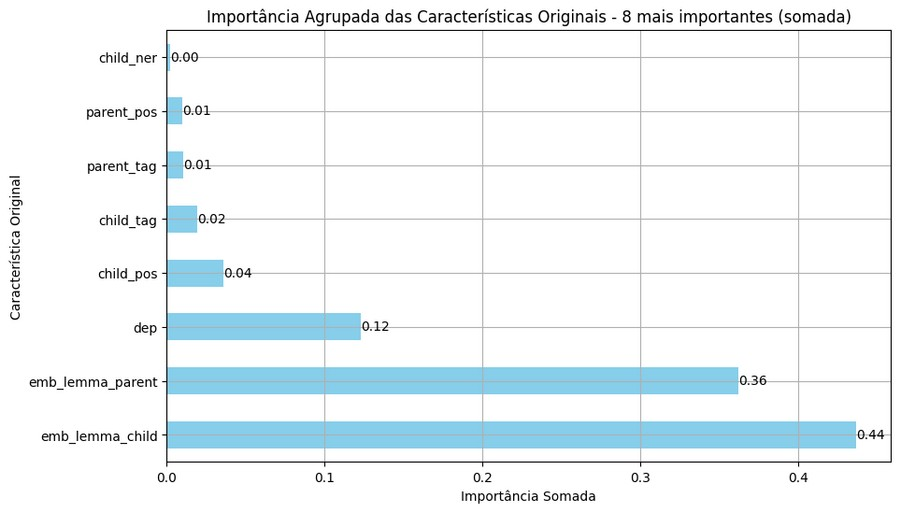
\includegraphics[width=\textwidth]{figure06.jpg}
  \caption{\emph{Features} mais relevantes para o Experimento 1.}
  \label{fig-06}
  \source{Elaborado pelos autores.}
  \end{minipage}
\end{figure}

\begin{figure}[htbp]
  \centering
  \begin{minipage}{.75\textwidth}
  
\includegraphics[width=\textwidth]{figure07.jpg}
  \caption{\emph{Features} mais relevantes para o Experimento 2.}
  \label{fig-07}
  \source{Elaborado pelos autores.}
  \end{minipage}
\end{figure}


Na \Cref{fig-06}, observa-se que os \emph{embeddings} dos lemas, tanto de
\emph{parent} quanto de \emph{child}, são particularmente significativos
para o modelo de classificação. No entanto, destaca-se que
\emph{embeddings} são as \emph{features} mais numerosas após a seleção.
Portanto, embora tenham uma grande soma de importância, individualmente,
sua relevância não é tão alta. Já na \Cref{fig-07}, além dos
\emph{embeddings} dos lemas, \emph{child\_tag}, \emph{child\_pos} e
\emph{dep} também se destacam. Nesse sentido, é possível inferir que, no
modelo criado, características de ordens morfossintáticas e sintáticas
são relevantes para a indicação dos papéis semânticos. Ressalta-se que
este tipo de observação é relevante em análises futuras, indicando quais
\emph{features} são mais relevantes em tarefas como a que foi
desenvolvida neste trabalho, além de contrapor o modelo teórico AMR que,
em tese, exclui esses níveis de conhecimento linguístico na
representação do significado e de sua estrutura argumental.

Por fim, foi empregado o método de \emph{shap values} para uma análise
mais profunda. Nesse método, conseguimos analisar como cada
\emph{feature} performa em função dos papéis semânticos observados. É
importante destacar que tal método se difere do
\emph{feature\_importance} por considerar a interação entre as
\emph{features} e a sua influência nas predições específicas. Vale
ressaltar que utilizamos apenas os \emph{shap values} para o conjunto de
treino, tendo em vista que o objetivo da análise é entender quais
padrões o modelo entendeu no seu treinamento como sendo mais
importantes. Para tanto, somaram-se os \emph{shap values} absolutos para
cada uma das \emph{features} originais e tirou-se a média de todas as
instâncias agrupadas pelo argumento para o Experimento 1 (\Cref{fig-08}) e o Experimento 2 (\Cref{fig-09}).

\begin{figure}[htpb]
  \centering
  \begin{minipage}{.75\textwidth}
  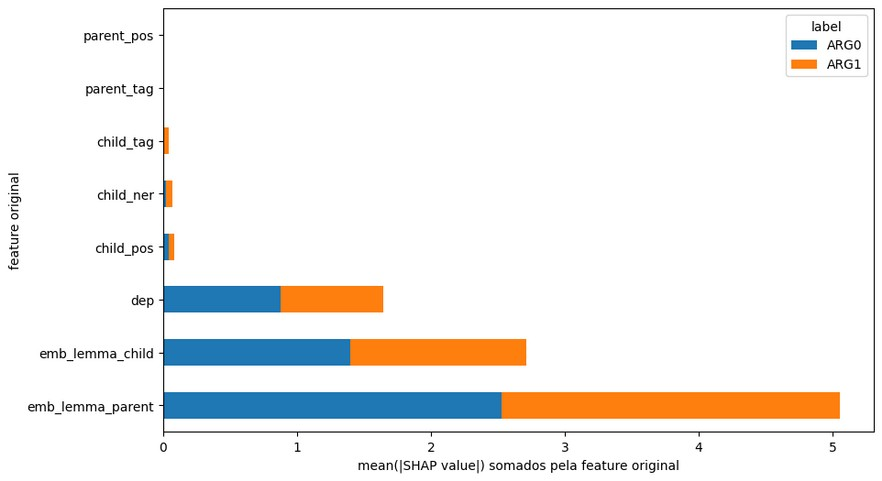
\includegraphics[width=\textwidth]{figure08.jpg}
  \caption{\emph{Features} mais relevantes para o Experimento 1 em função dos argumentos utilizando \emph{shap values}.}
  \label{fig-08}
  \source{Elaborado pelos autores.}
  \end{minipage}
\end{figure}

\begin{figure}[htbp]
  \centering
  \begin{minipage}{.75\textwidth}
  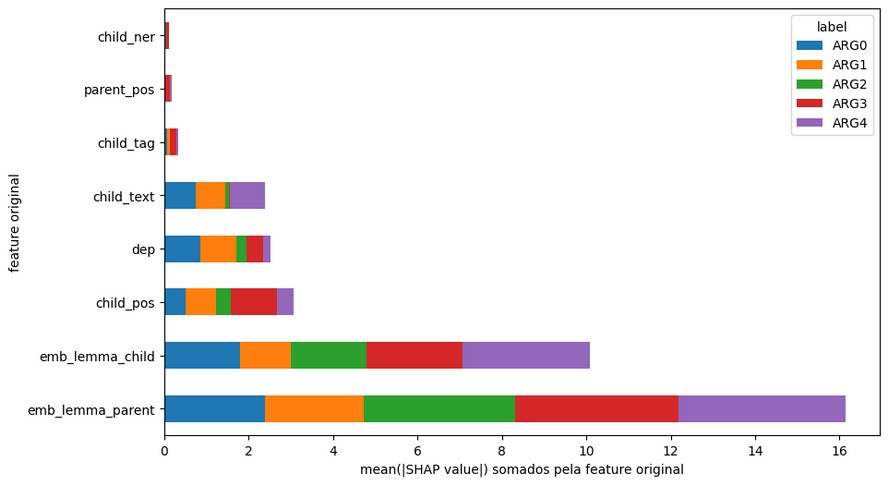
\includegraphics[width=\textwidth]{figure09.jpg}
  \caption{\emph{Features} mais relevantes para o Experimento 2 em função dos argumentos utilizando \emph{shap values}.}
  \label{fig-09}
  \source{Elaborado pelos autores.}
  \end{minipage}
\end{figure}


Na \Cref{fig-08}, evidencia-se que \emph{emb\_lemma\_parent} tem
discretamente maior relevância na classificação automática para Arg1 do
que Arg2, o que é inversamente proporcional para \emph{dep} e
\emph{emb\_lemma\_child}. Quanto a \emph{child\_tag}, \emph{child\_ner}
e \emph{child\_pos}, a relevância é bem baixa nesse cenário para as duas
classes analisadas; ao passo que \emph{parent\_pos} e \emph{parent\_tag}
não apresentaram qualquer relevância para nenhum dos dois papéis
semânticos. Quando o cenário de classificação é ampliado para os Args 0
a 4, o classificador recorre a algumas \emph{features} diferentes
daquelas utilizadas no primeiro experimento. Na \Cref{fig-09}, em especial,
tem-se que \emph{emb\_lemma\_parent} e \emph{emb\_lemma\_child} foram as
\emph{features} com maior relevância na classificação dos papéis
semânticos, sobretudo entre as classes Arg2, Arg3 e Arg4; ao passo que
\emph{child\_text}, que no experimento anterior não havia sido
utilizada, apresenta maior impacto para Arg0, Arg1 e Arg4.
\section{Considerações finais}\label{sec-consideraçõesfinais}

A partir da análise da vivência educacional descrita, visualizamos as interações propiciadas pelo novo \textit{ethos}, advindo do ciberespaço e da cultura digital, em especial, em contexto pandêmico, no qual as múltiplas semioses foram articuladas e propiciaram o exercício de consciência e agência dos alunos e dos professores.

Os participantes puderam olhar criticamente para as relações entre o eu, o outro e o meio ambiente em suas comunidades locais, problematizando questões socioambientais durante a pesquisa e o registro fotográfico, além de agir socialmente mediante a produção de vídeos e HQs que foram divulgados à comunidade em geral em eventos institucionais, bem como na internet.

Além disso, a técnica \textit{photovoice} aliada aos multiletramentos e à pedagogia psicodramática potencializou a mixagem de gêneros, mídias e linguagens, cara ao novo \textit{ethos} proveniente da cultura digital, na qual fontes, autorias e gêneros se articulam de forma rizomática.

Reconhecidos os limites deste texto e de todo trabalho educacional – que se estabelece na tênue linha educação-mercado –, esperamos que ele possa ajudar a pensar em alguns caminhos para o trabalho crítico com tecnologias digitais em sala de aula, de forma colaborativa e interdisciplinar e com foco em questões de linguagem.


\section{Agradecimentos}

Este trabalho foi realizado no âmbito do Centro de Inteligência
Artificial da Universidade de São Paulo (C4AI -
\url{http://c4ai.inova.usp.br/}), com o apoio da Fundação de Amparo à Pesquisa
do Estado de São Paulo (processo FAPESP \#2019/07665-4) e da IBM. Este
projeto também foi apoiado pelo Ministério da Ciência, Tecnologia e
Inovações, com recursos da Lei N. 8.248, de 23 de outubro de 1991, no
âmbito do PPI-Softex, coordenado pela Softex e publicado como Residência
em TIC 13, DOU 01245.010222/2022-44. Além disso, contou com o apoio
financeiro do Edital PRPPG-UFBA 010/2024 -- Programa de Apoio a Jovens
Professores(as)/Pesquisadores(as) 2024 -- e do Edital FAPESB/CNPq
004/2023 -- Programa Primeiros Projetos.



\printbibliography\label{sec-bib}
%conceptualization,datacuration,formalanalysis,funding,investigation,methodology,projadm,resources,software,supervision,validation,visualization,writing,review
\begin{contributors}[sec-contributors]
\authorcontribution{Jackson Wilke da Cruz Souza}[conceptualization,datacuration,formalanalysis,methodology,resources,software,supervision,validation,writing,review]
\authorcontribution{Pedro Semcovici}[datacuration,software,writing,review]
\authorcontribution{Thiago Alexandre Salgueiro Pardo}[conceptualization,resources,supervision,writing,review]
\end{contributors}
\end{document}
